\documentclass[]{scrartcl}

%Packages________________
\usepackage[normalem]{ulem}
\usepackage{cancel, xcolor}
\usepackage{parskip}
\usepackage{caption, subcaption}
\usepackage[Spanish,es-tabla,es-noshorthands]{babel}
\usepackage{newtxtext}
\usepackage[varvw]{newtxmath}
\usepackage{booktabs, colortbl, bigstrut, multirow, multicol}
\usepackage{url}
\usepackage{pgfplots}
\usepackage{graphicx}
\usepackage{amsmath}
\usepackage{tabularx}
\usepackage{floatrow}
\usepackage{float}
\usepackage{cancel}
\usepackage[spanish]{cleveref}
\usepackage{tikz}
\usetikzlibrary{arrows.meta}
\crefname{table}{tabla}{tablas}
\usepackage{wrapfig}
\usepackage{adjustbox}
\usepackage{geometry}
\usepackage{lipsum}
\usepackage{fancybox}
\geometry{
	top=2.4cm,
	bottom=2.4cm,
	left=2.3cm,
	right=2.3cm
}

\usepackage[
    backend=biber,
	citestyle=verbose-ibid,
    bibstyle=authoryear-icomp,
    natbib=true,
    url=true, 
    doi=true,
    eprint=false
]{biblatex}

\addbibresource{ref.bib}

%Commands________________
\newcommand\hcancel[2][black]{\setbox0=\hbox{$#2$}%strikeout
\rlap{\raisebox{.45\ht0}{\textcolor{#1}{\rule{\wd0}{1pt}}}}#2} 

\renewcommand\theequation{\Alph{equation}}

\renewcommand\thesubsection{\alph{subsection}}

%Titlepage_________________
\title{\vspace{-1.8cm} Circuitos - PEC 1}
\author{Álvaro Jerónimo Sánchez}
\date{}

%Document_____________
\begin{document}
\maketitle
\setcounter{section}{0}
\renewcommand{\tablename}{Tabla}


\section{Ejercicio 1}

En este circuito, se han nombrado los componentes como: \newline 
\begin{gather*}
	V_G=140V,\, I_G=8A,\, R_1=20\Omega ,\, R_2=6\Omega ,\, R_3=5\Omega
\end{gather*}

\subsection{Voltaje en los nodos A y B}

Estos nodos en realidad son el mismo nodo, ya que están conectados sin ningún componente entre ellos, por lo que se se cumple que $V_A=V_B$. Aplicando la primera Ley de Kirchhoff:
\begin{gather*}
	0=\frac{V_A-V_G}{R_1}+\frac{V_A-0}{R2}+\frac{V_A-0}{R_3}-8\, A\\
	0= 3V_A -420 + 22V_A -480 \Rightarrow V_A = \frac{900}{25}\\
	\boxed{V_A=V_B=36\, V}
\end{gather*}

\subsection{Potencia disipada en cada resistencia}

Este apartado se puede resolver con una aplicación directa de la definición de la potencia y usando Ohm:
\begin{gather*}
	P=\frac{dW}{dt}=V\frac{dq}{dt}=VI=\frac{V^2}{R}\\
	P_{R1}=\frac{(V_G -V_A)^2}{R_1}=\boxed{540.8\, W}\;
	P_{R2}=\frac{V_A ^2}{R_2}=\boxed{216.0\, W}\;
	P_{R3}=\frac{V_A ^2}{R_3}=\boxed{259.2\, W}\;
\end{gather*}

\section{Ejercicio 2}

\begin{wrapfigure}{r}{0.4\textwidth}
\centering
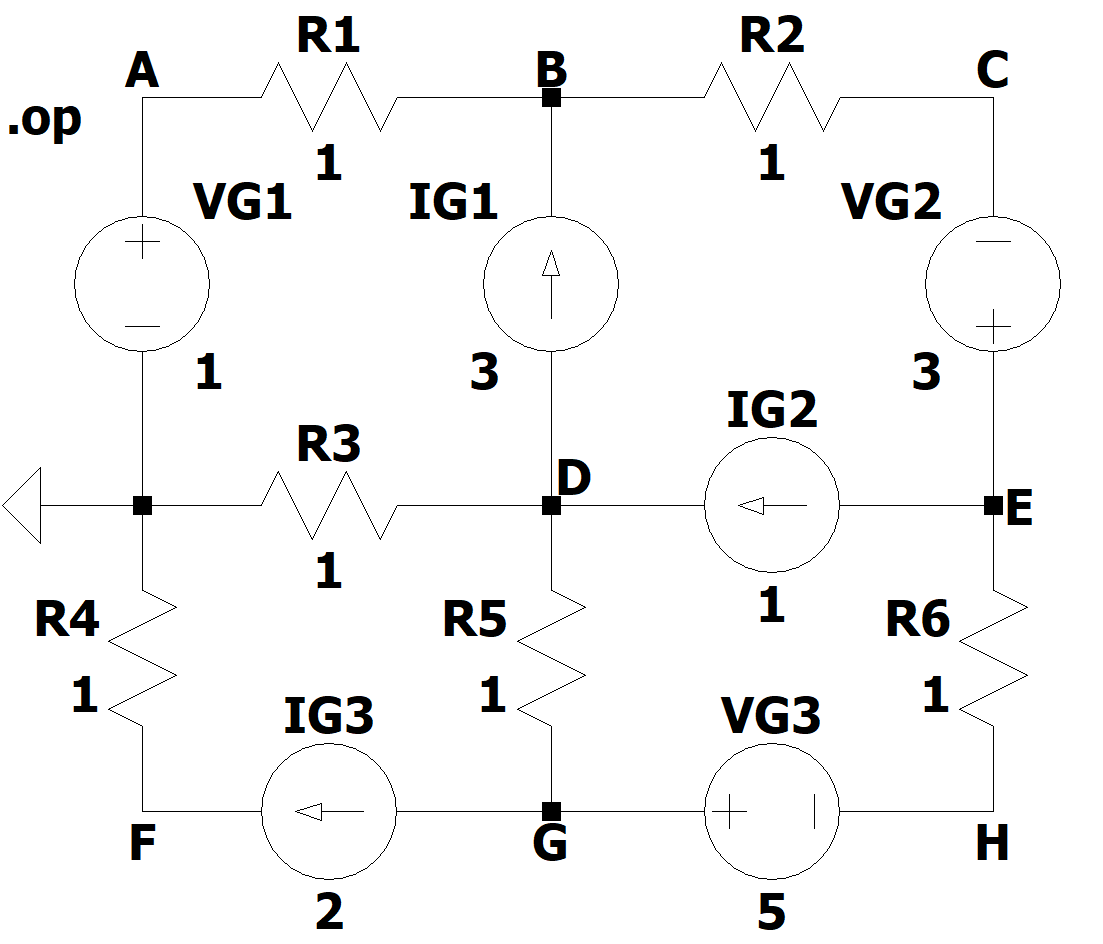
\includegraphics[width=0.95\columnwidth]{../2.png}
\end{wrapfigure}

\textit{Para ver la nomenclatura usada para cada compuesto/nodo, ver la imagen adjunta a la derecha}. Se ha colocado tierra en el nodo conectado a $V_{G1}$, $R_3$ y $R_4$. Se han generado dos supernodos en $V_{G2}$ y $V_{G3}$.

\subsection{Corriente de cada R}

Se ha planteado un sistema de ecuaciones empleando la primera Ley de Kirchhoff, que posteriormente se ha reducido con las condiciones intrínsecas de los supernodos $V_E - V_C = 3\, V$ ; $V_G-V_H=5\, V$. Se ha planteado una matriz que se ha resuelto por Gauss. Las ecuaciones de los nodos son (en orden alfabético): \clearpage
\begin{equation*}
	\left\{
	\begin{array}{l}
		V_A=1\\
		0=V_C-V_B+1+V_E-V_H\\
		0=V_D-0+3-1+V_D-V_G\\
		0=V_F-0-2 \Rightarrow V_F=2\\
		0=V_H -V_E+2+V_G-V_D
	\end{array}
	\right. \leadsto \left\{
	\begin{array}{l}
		2V_B-V_E=1\\
		-V_B+2V_E-V_G=-3\\
		2V_D-V_G=-2\\
		-V_D-V_E+2V_G=3
	\end{array}
	\right.\Rightarrow \left[
	\begin{array}{cccc|c}
		2&0&-1&0&1\\0&2&0&-1&-2\\-1&0&2&-1&-3\\0&-1&-1&0&3
	\end{array}
	\right]
\end{equation*}

Que al resolverla por Gauss-Jordan nos da (en voltios):
\begin{gather*}
	V_A=1\, ;\; V_B=-0.2\, ;\; V_C=-4.4\, ;\; V_D=-0.8\, ;\; V_E=-1.4\, ;\; V_F=2\, ;\; V_G=0.4\, ;\; V_H=-4.6\, ;\; 
\end{gather*}

Hallamos las intensidades aplicando la Ley de Ohm. Aquellas que salgan con signo negativo es que van en sentido \textbf{contrario} al planteado en la diferencia:
\begin{table}[H]
\centering
%\def\arraystretch{1.5}
\begin{tabular}{|c|c|}  \hline
$I_{R1}=V_A-V_B=1.2$ & $I_{R4}=V_F-0=2$ \\ \hline
$I_{R2}=V_B-V_C=4.2$ & $I_{R5}=V_G-V_D=1.2$ \\ \hline
$I_{R3}=V_D-0=-0.8$ & $I_{R6}=V_E-V_H=3.2$ \\ \hline
\end{tabular}
\end{table}

\subsection{Potencia de las fuentes}

Es una aplicación directa de $P=VI$. Si el resultado es negativo, quiere decir que aporta potencia en sentido \textbf{opuesto} a la corriente (``absorbe''). Los resultados (en vatios) son los siguientes:
\begin{table}[H]
\centering
%\def\arraystretch{1.5}
\begin{tabular}{|c|c|}  \hline
$P_{VG1}=1(1-0)=1$ & $P_{IG1}=(-0.8+0.2)3=-1.8$ \\ \hline
$P_{VG2}=3(-1.4+4.4)=9$ & $P_{IG2}=(-1.4+0.8)1=-0.6$ \\ \hline
$P_{VG3}=5(0.4+4.6)=-25$ & $P_{IG3}=(0.4-2)2=-3.2$ \\ \hline
\end{tabular}
\end{table}

\section{Ejercicio 3}

\begin{wrapfigure}[8]{l}{0.4\textwidth}
\centering
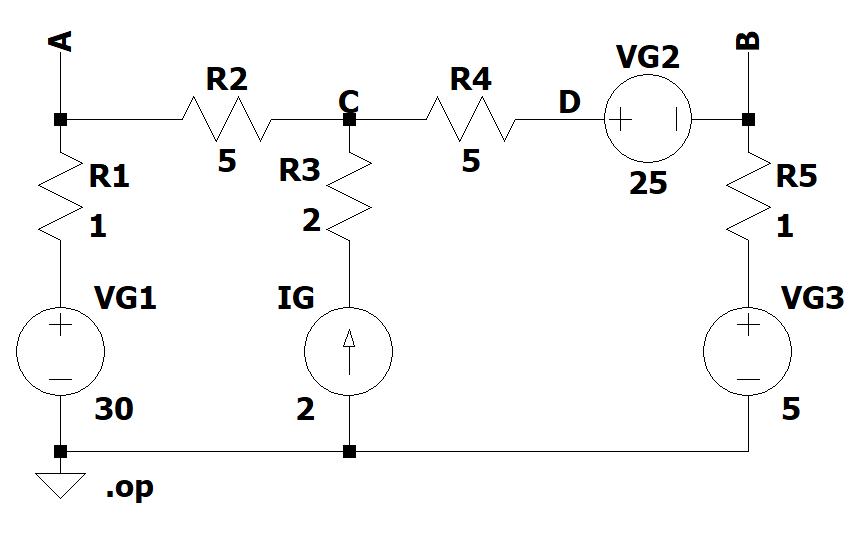
\includegraphics[width=0.95\columnwidth]{../3.png}
\end{wrapfigure}

\subsection{Voltaje de Thévenin}

El voltaje de Thévenin será el voltaje entre los nodos A y B. Planteamos las ecuaciones de nodos teniendo en cuenta que hay un supernodo B-D, por lo que $V_D-V_B=25\, V$. Posteriormente, sustituimos en el sistema y planteamos una matriz para solucionar por Gauss:
\begin{gather*}
	\left\{
	\begin{array}{l}
		0=V_A-V_{G1}+\frac{V_A-V_C}{R_2}\\
		0=\frac{V_C-V_A}{R_2}-I_G+\frac{V_C-V_D}{R_4}\\
		0=\frac{V_D-V_C}{R_4}+V_B-V_{G3}
	\end{array}
	\right. \leadsto \left[
	\begin{array}{ccc|c}
		6&-1&0&150\\-1&2&-1&10\\0&-1&6&150
	\end{array}
	\right]
\end{gather*}

Tras resolver por Gauss y sustituir, obtenemos (en voltios):
\begin{gather*}
	V_A=31\, ; \; V_B=6\, ; \; V_C=36\, ; \; V_D=31 
\end{gather*}
Por tanto: $\boxed{V_{th}=V_A-V_B=25\, V}$ \clearpage

\subsection{Resistencia de Thévenin}

Como las fuentes son ideales, para el circuito equivalente se cortocircuitan las fuentes de voltaje y se abren las de corriente. Asociando las resistencias restantes (y teniendo en cuenta los nodos A y B para determinar que las resistencias adyacentes no están en serie), obtenemos:
\begin{gather*}
	\frac{1}{R_{th}}=\frac{1}{10}+\frac{1}{2}\Rightarrow R_{th}=\frac{1}{0.6} = \boxed{1.67\, \Omega}
\end{gather*}

\subsection{Potencia máxima disipada}

La potencia máxima que disipará la carga se dará cuando $R_L=R_{th}$. Por lo que, aplicando la definición de la potencia:
\begin{gather*}
	P=I^2 R = \left( \frac{V_{th}}{R_{th}+R_L} \right)^2 R_{th}=\frac{V^2}{4R^2 _{th}}R_{th}=\boxed{93.56\, W}
\end{gather*}

\section{Ejercicio 4}

\begin{wrapfigure}{r}{0.4\textwidth}
\centering
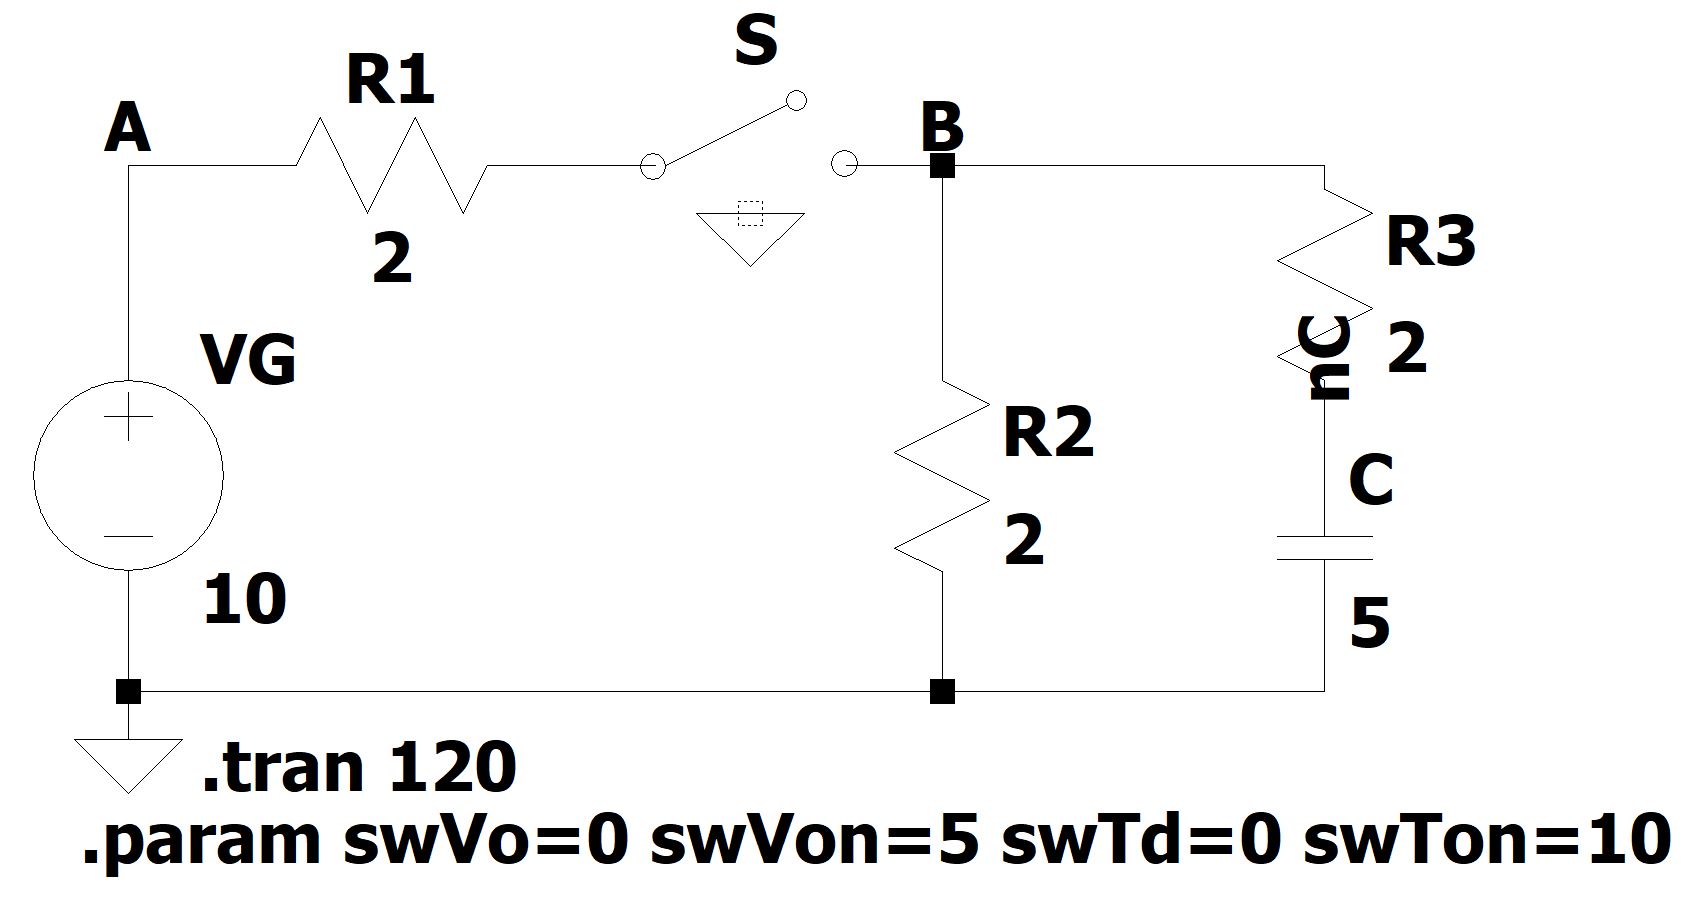
\includegraphics[width=0.95\columnwidth]{../4.png}
\end{wrapfigure}

El componente $S$ se trata de un interruptor activado por voltaje, que es el único tipo que \textit{LTspice} ofrece. Se ha elegido que este se cerrará mientras reciba un voltaje de 5 V.Se ha representado con un subcircuito para mejor claridad visual, que se puede encontrar adjunto en el apéndice (\cref{fig:sw}) con la explicación de cada parámetro.

\subsection{V para t $>$ 0}

La fórmula del voltaje con el tiempo tendrá una forma $v(t)=A+Be^{-\frac{t}{\tau}}$, siendo $A+B$ la condición inicial, y $A$ la solución estacionaria. Como empieza descargado, $A+B=0$. Con fin de hallar la solución estacionaria, se ha hecho el equivalente Thévenin. Se ha tenido en cuenta que la rama del condensador quedará abierta para $t\rightarrow\infty$, y planteado la ecuación del nodo tenemos:
\begin{gather*}
	0=\frac{V_A-10}{2}+\frac{V_A}{2} \rightarrow V_{est}=V_A-0=5\, V
\end{gather*}
A continuación, para hallar $\tau$ con la $R_{th}$, cortocircuitamos la fuente y asociamos resistencias. Sustituimos en la ecuación de $v(t)$.
\begin{gather*}
	\tau=\left(\frac{1}{\frac{1}{2}+\frac{1}{2}}+2\right)C=15\, s\\
	\boxed{v(t)=5-5e^{-\frac{t}{15}}\, V}
\end{gather*}

\subsection{V para t $>$ 10}

AL abrir el interruptor, la fuente y $R_1$ quedan desconectados del circuito. EL condensador se descargará, proporcionando voltaje en la dirección contraria. Planteamos la ecuación de $v_{10}(t)$ de forma análoga y resolvemos $\tau$ tras asociar las resistencias. Tenemos en cuenta que $A=0$, ya que en $t\rightarrow\inf$ el condensador se descarga completamente; y que $A+B=v(10)$, que será la condición inicial (a los 10 segundos) dictada por la ecuación hallada en el apartado anterior.
\begin{gather*}
	A+B=v(10)=2.43\, V\; ; \; \tau=(R_2+R_3)C=20\, s\\
	\boxed{v_{10}(t)=2.43e^{-\frac{t}{20}}\, V}
\end{gather*}

\subsection{Gráfica voltaje-tiempo}

Para realizar esta gráfica se ha usado \textit{LTspice} y se han marcado los dos puntos pedidos. Podemos observar que coincide con los resultados teóricos hallados.
\begin{figure}[h]
\centering
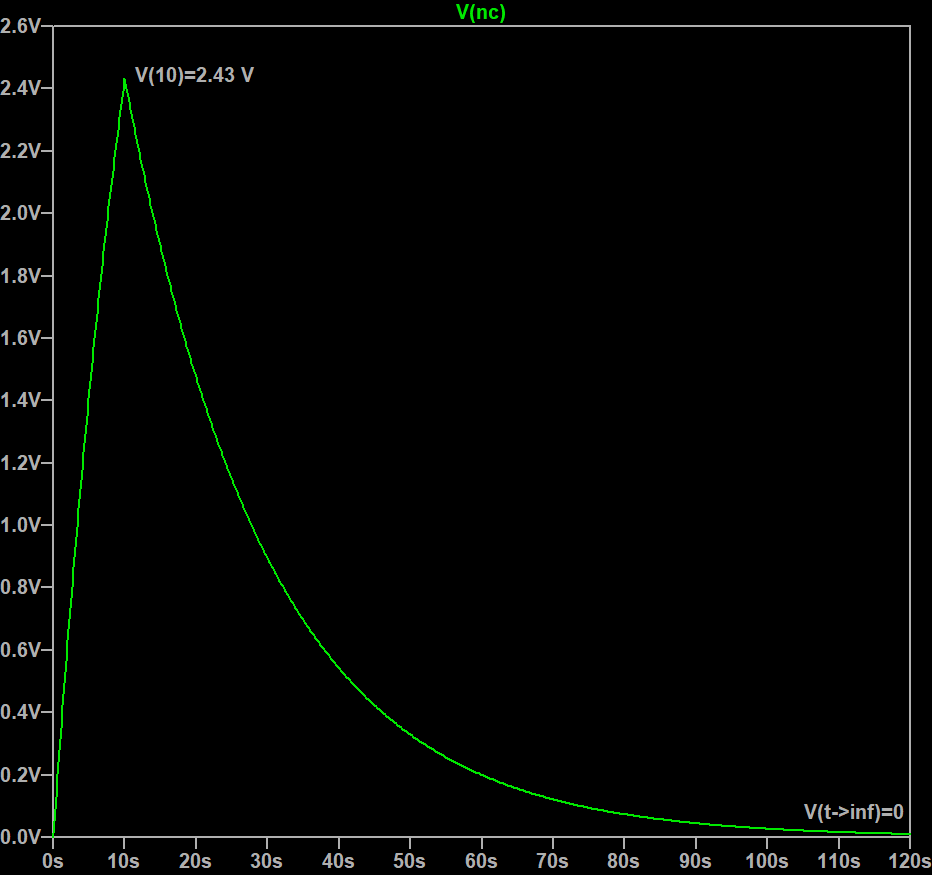
\includegraphics[width=0.6\columnwidth]{../4-g.png}
\end{figure}

\section{Ejercicio 5}

En este ejercicio hay un supernado en la fuente de corriente alterna de la rama derecha, al nodo no nombrado conectado a su terminal negativo se le ha llamado $D$. Teniendo en cuenta este supernodo ($V_C-V_D=5\, V$), además de la dependencia de la fuente de corriente central, planteamos las ecuaciones de los nodos y resolvemos la matriz del sistema tras sustituir para hallar las impedancias:
\begin{gather*}
	Z_L=j\; ; \; Z_C=-j\\
	\left\{
	\begin{array}{l}
		0=-10-\frac{V_A+V_C}{j}\\
		0=V_B-V_A+2\frac{V_D}{2}\\
		0=\frac{V_C-V_B}{j}+\frac{V_D}{2}
	\end{array}
	\right.	\leadsto
	\left\{
	\begin{array}{l}
		0=-V_A+V_C-10j\\
		0=-V_Aj+V_B(j+1)-5j\\
		0=-2V_B+3V_Cj-5j		
	\end{array} 
	\right. \Rightarrow
	\left[
	\begin{array}{ccc|c} 
		-1&0&1&-10j\\ -j&(j+1)&0&-5j\\ 0&-2&-3j&-5j		
	\end{array}
	\right]
\end{gather*}
Tras resolver la matriz, hallamos que:
\begin{gather*}
	\boxed{V_A=5j}\; ; \; \boxed{V_B=-5}\; ; \; \boxed{V_C=5j}\;
\end{gather*}

\clearpage

%_____________________________

\appendix
\textbf{APPENDIX}

\begin{figure}[h]
\centering
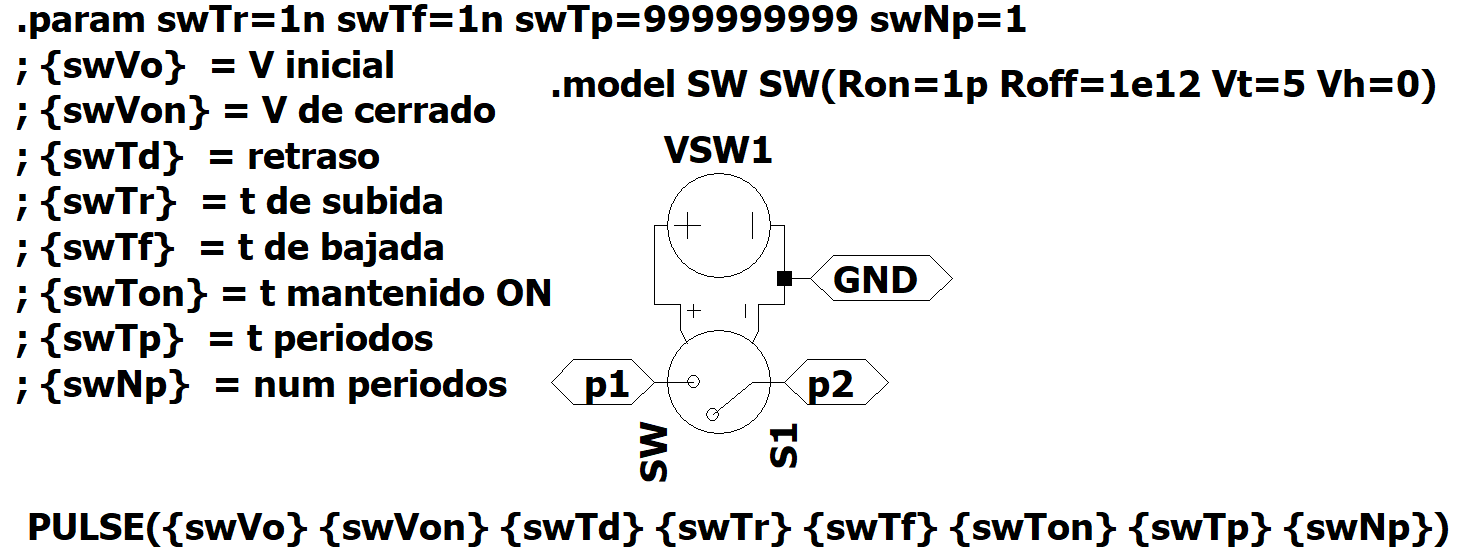
\includegraphics[width=0.6\columnwidth]{../sw.png}
\label{fig:sw}
\end{figure}

\vspace{2cm}
\begin{center}
\setlength{\fboxsep}{0.5cm}
\shadowbox{\begin{minipage}{10.5cm}
\textbf{Declaración de Autoría}\\

El alumno
Álvaro Jerónimo Sánchez
, con DNI número 
09847051S
, declara que es el autor único e individual de este trabajo.\\

\vspace{3cm}
Fdo:

\end{minipage}}
\end{center}


\end{document}